\documentclass[11pt]{article}
\title{Geant4 Benchmark Analysis:\\ Al cube and He cylindrical chamber}
\author{Shaun Marshall}
\date{\today}
\usepackage{abstract}
\usepackage{multicol}
\usepackage{anysize}
\usepackage{graphicx}
\usepackage{url}
\usepackage{float}

% Figures within a column...
\makeatletter
\newenvironment{tablehere}
{\def\@captype{table}}{}
\newenvironment{figurehere}
{\def\@captype{figure}}{}
\makeatother

\marginsize{0.75 in}{0.75 in}{0.75 in}{0.75 in}
\begin{document}
\maketitle

\begin{abstract}\emph{
This experiment analyzes a setup of interest, firing collimated protons and neutrons in the range of $10^0-5\cdot10^8\ eV$ at an aluminum box 50 cm away of side 5, 10, and 25 cm, 50 cm, in front of a cylindrical container of helium 50 cm further.  The encoded tasks which assess and characterize the scenario include an energy deposition map, charge displacemnent map, and particle creation probabilities tables.  Results are comparable to empirical studies of proton dosimetry and demonstrate validity of Geant4 theoretical modeling.
}\end{abstract}

\begin{multicols}{2}

\section{Introduction}

Geant4 is a Monte Carlo simulation software written in C++, used by many leading research institutions of nuclear and particle physics\cite{?}.  Components of definition, runtime and analysis are compiled separately as classes located in header files; such generalized object-variables are well-suited for precise and fully customizable geometric and analytical specifications.

\section{Procedure}

1 million simulated events of collimated protons and neutrons were fired 50 cm to an Aluminum block in a vacuous world, which lie 50 cm in front of a cylindrical He gas chamber centered in line with the block vertically, perpendicular to the cylinder's long axis (fig~\ref{fig:schematic}).  This geometry was iterated for the 5, 10 and 25 cm side lengths of the block.  Energy deposition and net charge transfer by millimeter were recorded and normalized per primary.  Proton and neutron production combinations are found in time with gamma ray creation.

\vspace{0.25 cm}
\begin{figurehere}
\centering
\resizebox{\columnwidth}{!}{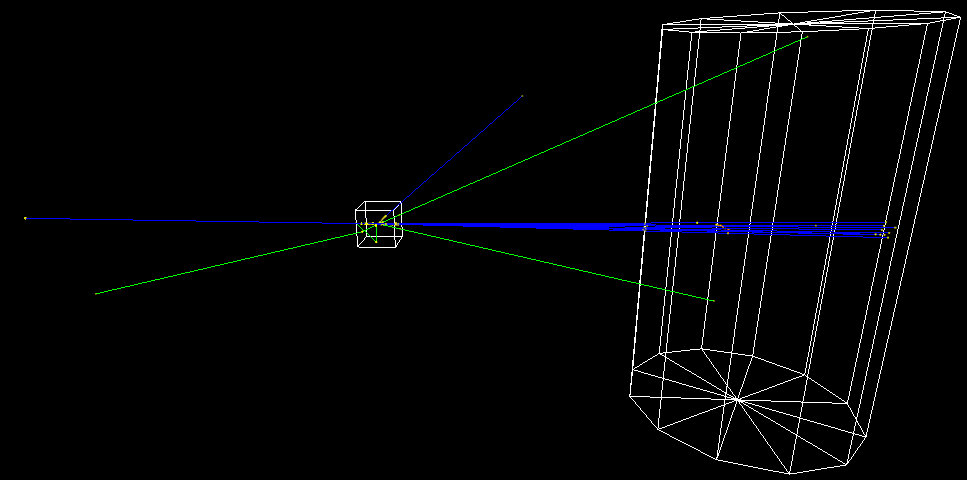
\includegraphics{../testrun.png}}
\caption{\small \emph{Schematic of constructed detector geometry with sample event, using Geant4 OpenGL visualization.}}
\label{fig:schematic}
\end{figurehere}
\vspace{0.25 cm}

The FTFP\_BERT physics list was utilized\cite{Geant4:physicsList}, with track cuts at a 10 micron minimum step legnth.  Primary particle energies range from $1$ to $5\cdot10^x$, where $x:\mathcal{Z}\in[0,8]$.

\subsection{Energy Deposition Tracking}

To acquire an energy deposition map of proton and neutron events in this physical setup, a script was introduced into the UserSteppingAction class.  This script acquired the position (in mm) and energy (in MeV) of every collision (G4Step) per event.  A UserRunAction method took averages ofenergy depositions throughout the 1150 mm world per bin, event, primary energy (G4Run) and geometry.

\subsection{Charge Deposition Tracking}

The charge deposition map for the proton and neutron events also utilized a UserSteppingAction script to obtain spatial values of charge displacement.  Dividing the world into (mm) bins, charge values of particles which gained momentum per event are subtracted from the bin of track vertex and added to the bin of track end.  The end of each G4Run included an averaging of the net charge per bin, event, energy and geometry; this net charge signature depicts the average polarization of the detectors.

\subsection{Particle Production Tracking}

Probably particle production matrices $P(n,m)$ were constructed by probing each G4Step which marked the end of a secondary particle's track for the particle name.  Gamma rays (indicitive of secondary electron production), as well as $n\times m$ combinations of secondary protons and neutrons for $n,m:\mathcal{Z}\in[1,5], \lq 5+$' were tallied per event.  Each G4Run ended by averaging the productions combinations by event per energy and geometry, normalizing the result such that $\sum_n \sum_m P(n,m) = 1$.

\section{Discussion}

\section{Conclusion}

\section{References}
\begin{thebibliography}{99}

\bibitem[1]{Geant4:physicsList}
\lq\lq Use cases - Reference Physics Lists." \\
Geant4 Online User Support. \\
\url{http://www.geant4.org/geant4/support/proc_mod_catalog/physics_lists/useCases.shtml}
 
\end{thebibliography}

\end{multicols}
\end{document}
